% In system (10), vary r from 0 to 2. Which bifurcations occur?
% At which numerical values do you find steady states and limit cycles of the system?
% Now vary r from 2 to 4. What happens?
% Plot and discuss a bifurcation diagram for r between 0 and 4.
% Visualize a single trajectory of the Lorenz system starting at x0 = (10, 10, 10), discuss the results.
% Test initial condition dependence by plotting another trajectory.
% At what time is the difference between the points on the trajectory larger than 1?
% Change to ρ = 0.5 and again compute and plot the two trajectories. Is there a bifurcation?
% Short description of the setup in the report?

Now, our goal is to study chaos in dynamical systems using two systems. \\

\textbf{Part 1:} For this part, we focus on a very simple equation of "logistic map" given by the equation (1) where x is the current state, r is the growth rate, and $x_{n+1}$ is the next state with $x \in [0,1] \; \text{and} \; r \in (0,4]$
\begin{align}
    x_{n+1} = rx_n(1 - x_n), \quad n \in \mathbb{N}
\end{align}

\begin{itemize}
    \item \textbf{Vary r from 0 to 2:} For this task, we plotted the logistic map for four different values of x = [0.25, 0.5, 0.75, 0.9] and r values between 0 and 2 with 0.1 increments on 50 timesteps. Figure \ref{fig:Logistic_map_0_2} shows two outputs of a logistic map for different values of r and x. Looking at these plots closely, we can see that for values of r below 1, the steady state gets down to zero or dies out. We can look at this with the analogy of x being the rabbit population and r being the reproduction rate. So, if the reproduction rate is too low (r \textless 1), the rabbit population dies out as can be seen in figure \ref{fig:r_0_1}. But if the reproduction rate is higher (1 \textless r \textless 2), the population reaches a constant value (not zero) or there is no change in the population and the rate of death is equal to the rate of birth as can be seen in figure \ref{fig:r_0_2}. The population either increases or decreases(x=0.5, r=1.4) but reaches a constant steady state.

\begin{figure}[H]
    \centering
    \begin{subfigure}[b]{\textwidth}
        \centering
        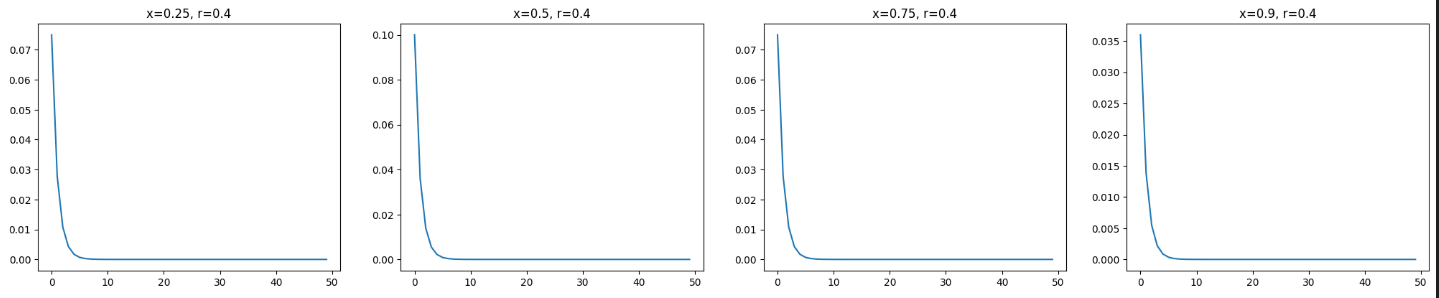
\includegraphics[width=\textwidth]{images/ex4task4_r_0_1.png}
        \caption{0\textless r\textless 1}
        \label{fig:r_0_1}
    \end{subfigure}
    \hfill
    \begin{subfigure}[b]{\textwidth}
        \centering
        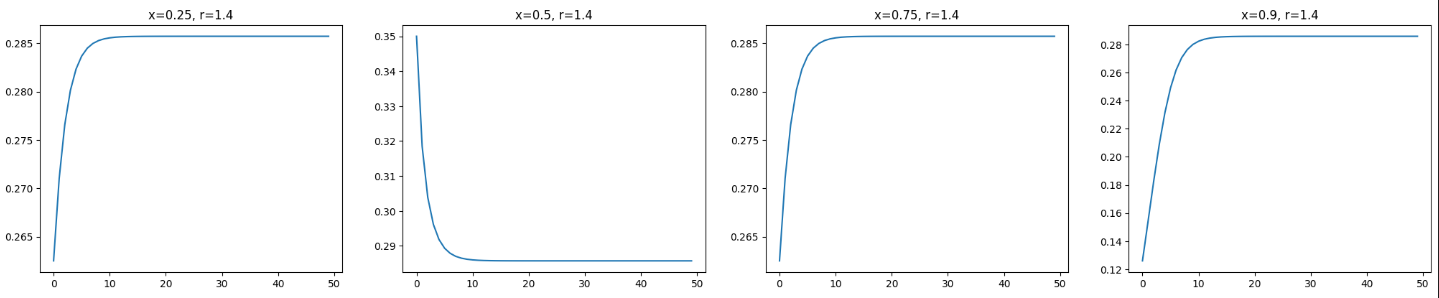
\includegraphics[width=\textwidth]{images/ex4task4_r_1_2.png}
        \caption{1\textless r \textless2}
        \label{fig:r_0_2}
    \end{subfigure}
    \caption{Logistic map for different values of r and x}
    \label{fig:Logistic_map_0_2}
\end{figure}

We can observe the same in the bifurcation diagram \ref{fig:bifurcation_0_2}. For r values below 1, the function dies out or becomes 0, while for r values between 0 and 1, the function has a constant not zero value. Also, there are no bifurcations in this range of r.

\begin{figure} [H]
    \centering
    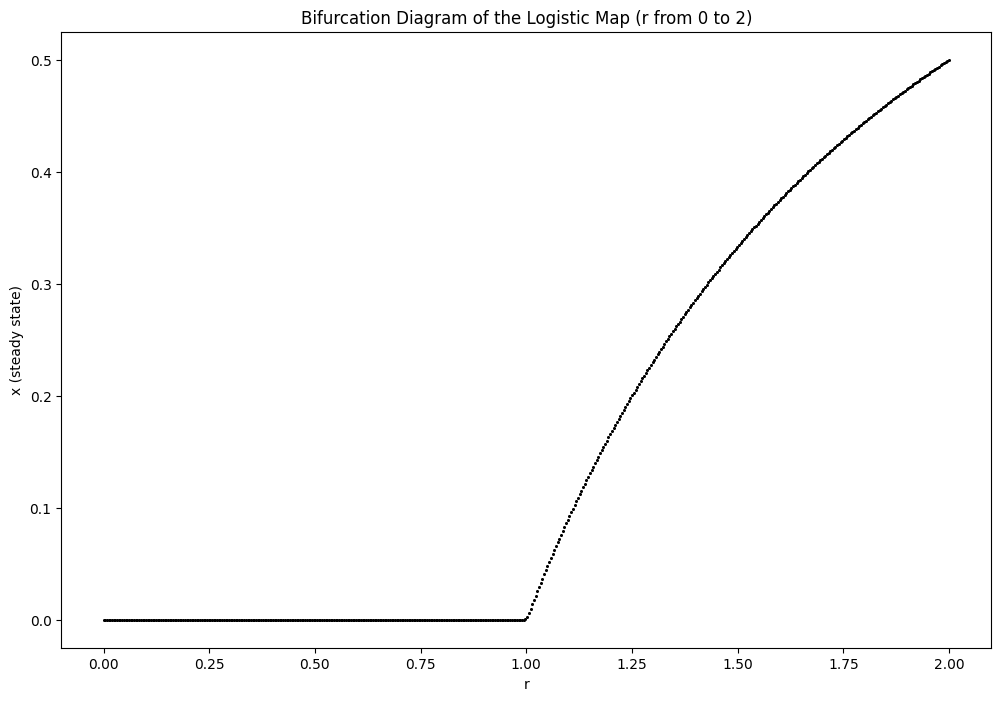
\includegraphics[width=0.4\textwidth]{images/ex4task4_bifurcation_0_2.png}
    \caption{Bifurcation Diagram for $r$ between 0 and 2}
    \label{fig:bifurcation_0_2}
\end{figure}

    \item \textbf{Vary r from 2 to 4:} We repeat the same experiment for r values between 2 to 4 and observe the results. We use the same four different values of x = [0.25, 0.5, 0.75, 0.9] and plotted the logistic map for 100 timesteps. Figure \ref{fig:Logistic_map_2_4} shows three outputs of the logistic map for different values of r and x. We can observe the changes in these figures now. For the r value between 2 and 3 as shown in figure \ref{fig:r_2_3}, the population first fluctuates before becoming constant (not zero). For r values between 3 and roughly 3.5, as shown in figure \ref{fig:r_3_35}, the population permanently oscillates between two values. Here, we can say that a bifurcation has occurred. If we keep increasing r and look at the graph after 3.5 as seen in figure \ref{fig:r_35} (here for r=3.6), the graph starts oscillating rapidly between multiple values. We can now say that the values are pseudo-random (as it is deterministic) or, in other terms, that chaos has ensued.

\begin{figure}[H]
    \centering
    \begin{subfigure}[b]{0.7\textwidth}
        \centering
        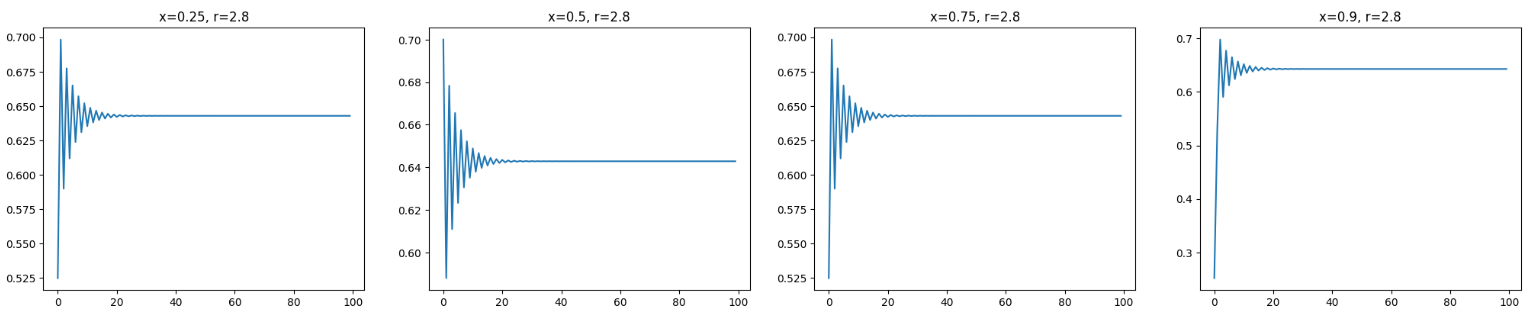
\includegraphics[width=\textwidth]{images/ex4task4_r_2_3.png}
        \caption{2\textless r\textless 3}
        \label{fig:r_2_3}
    \end{subfigure}
    \hfill
    \begin{subfigure}[b]{0.7\textwidth}
        \centering
        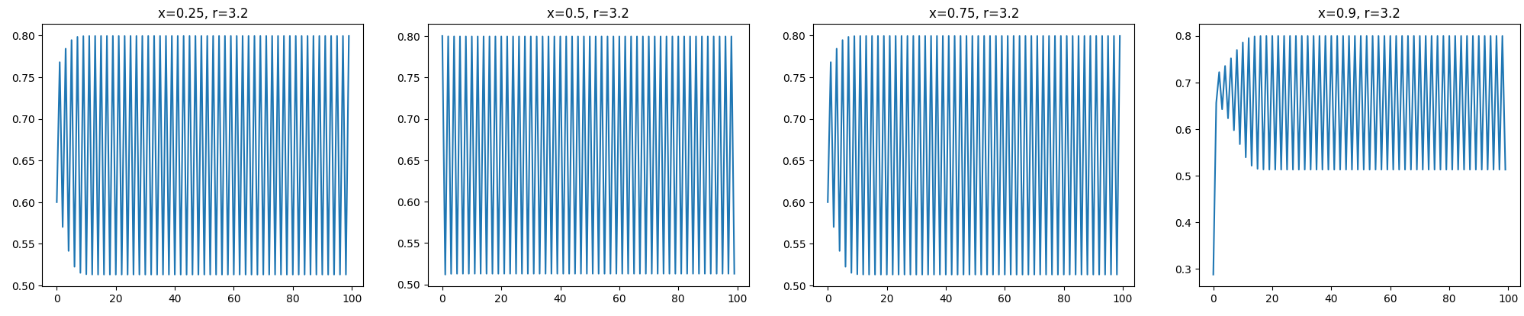
\includegraphics[width=\textwidth]{images/ex4task4_r_3_35.png}
        \caption{3\textless r \textless3.5}
        \label{fig:r_3_35}
    \end{subfigure}
        \begin{subfigure}[b]{0.7\textwidth}
        \centering
        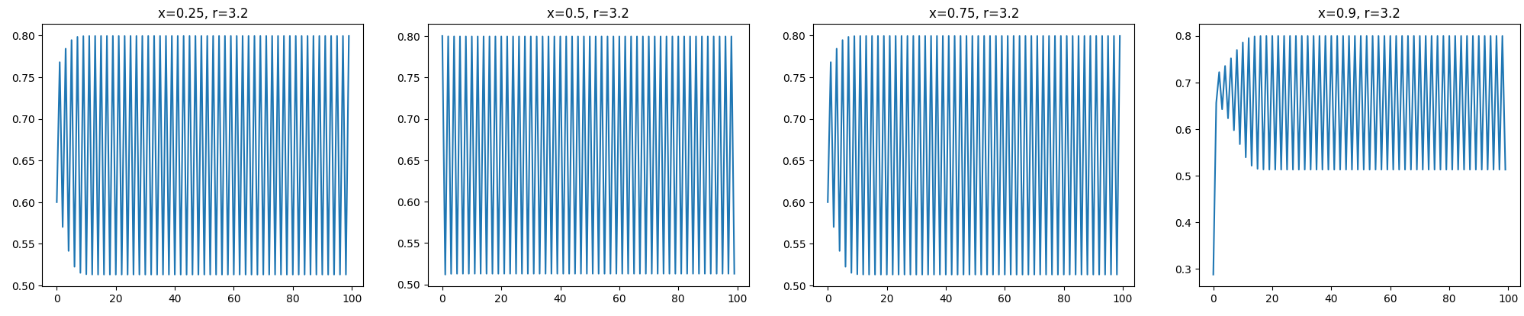
\includegraphics[width=\textwidth]{images/ex4task4_r_3_35.png}
        \caption{3.5\textless r}
        \label{fig:r_35}
    \end{subfigure}
    \caption{Logistic map for different values of r and x}
    \label{fig:Logistic_map_2_4}
\end{figure}

We can observe the same in the bifurcation diagram \ref{fig:bifurcation_2_4}. For values between 2 and 3, we only see one steady state. As the r value increases beyond 3, the steady state bifurcates into two. Increasing r further beyond 3.5, it further bifurcates into 4 values, and then rapidly into 8, 16, 32, etc. We can say that the values are now chaotic and pseudo-random.

\begin{figure} [H]
    \centering
    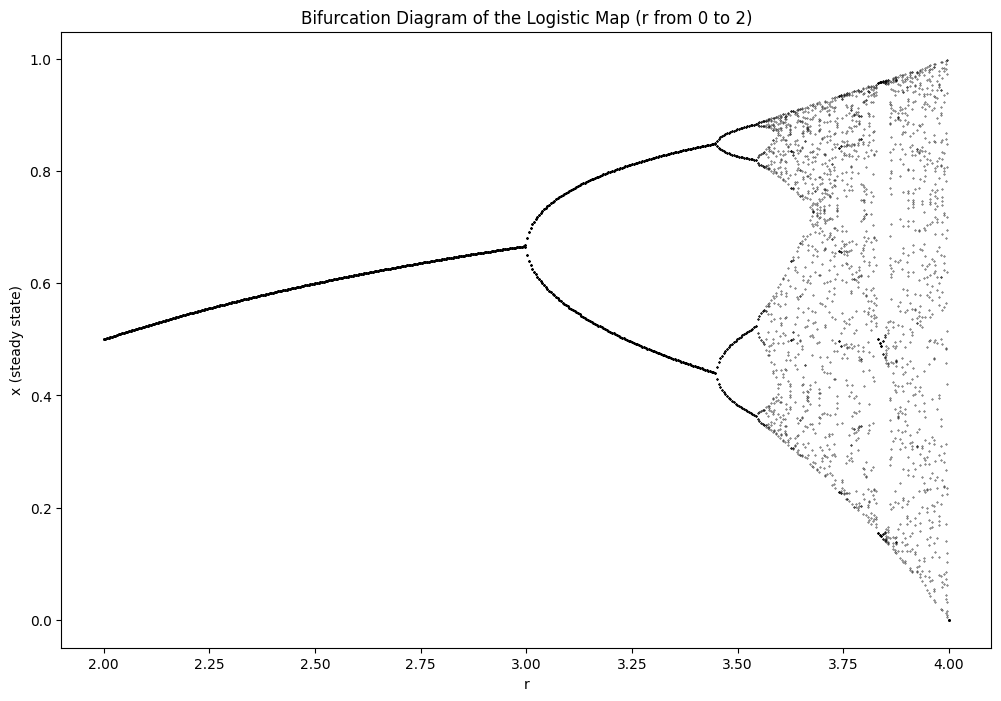
\includegraphics[width=0.5\textwidth]{images/ex4task4_bifurcation_2_4.png}
    \caption{Bifurcation Diagram for $r$ between 2 and 4}
    \label{fig:bifurcation_2_4}
\end{figure}

\item \textbf{Bifurcation diagram between 0 and 4}: We plotted the bifurcation diagram for x=0.5 for r values between 0 and 4, as shown in Figure \ref{fig:bifurcation_0_4}. We utilized the function \texttt{plot\_bifurcation\_diagram} in \texttt{utils.py} to generate the bifurcation diagrams for this part and the previous two sections. To observe the final state of the system, we ran the logistic map for a specific number of timesteps to get rid of transient values and selected only the last few values (steady state) for plotting. We can again see that for r values between 0 and 1, we get 0 as the steady state, for values between 1 and 3, we can see a non-zero steady state, after 3, the graph bifurcates into two values. Increasing r beyond 3.5, the values bifurcate continuously into 4, 8, 16, etc. We can say that the values are now chaotic. One of the interesting observations that can be seen in the graph is that for r values roughly around 3.8, the graph shows non-chaotic behaviour with steady state oscillating between 3 distinct values. But with a further increase in r, the steady state again becomes chaotic.



\begin{figure} [H]
    \centering
    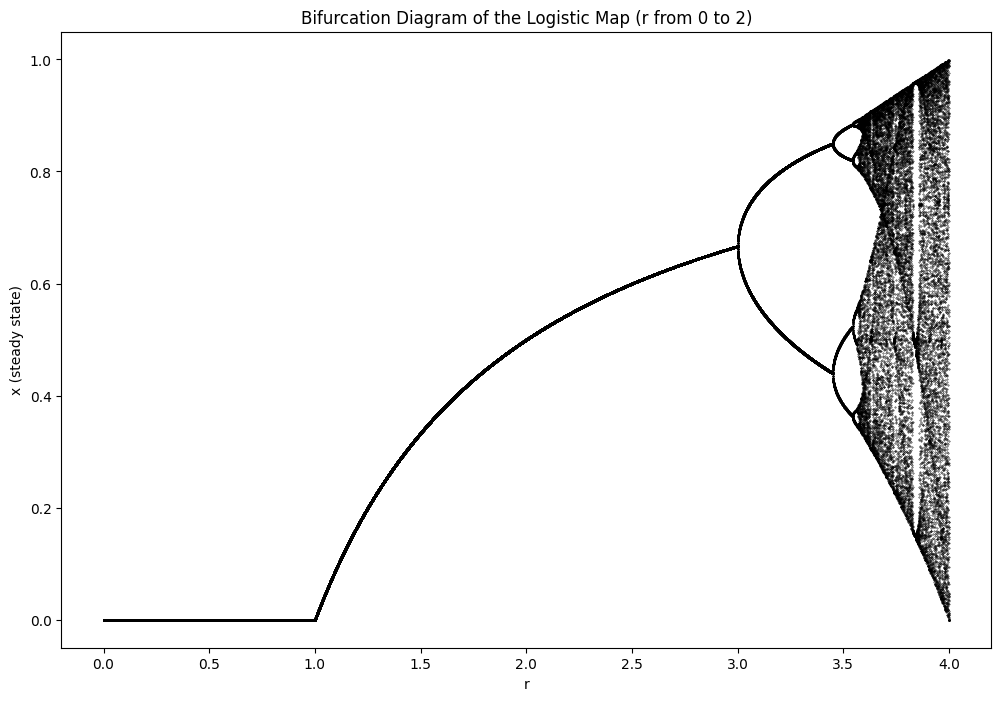
\includegraphics[width=0.5\textwidth]{images/ex4task4_bifurcation_diagam_final.png}
    \caption{Bifurcation Diagram for $r$ between 0 and 4}
    \label{fig:bifurcation_0_4}
\end{figure}

\end{itemize}

\textbf{Part 2:} For this part, we continue our exploration of chaotic dynamics using another famous attractor known as the Lorenz attractor \cite{lorenz1963}, which is a strange attractor with chaotic dynamics. The system is represented by the following equations which we implemented in the function \texttt{lorenz\_system()}:
    \begin{align}
        \frac{dx}{dt} &= \sigma(y - x) \\
        \frac{dy}{dt} &= x(\rho - z) - y \\
        \frac{dz}{dt} &= xy - \beta z
    \end{align}

   \begin{itemize}
       \item  \textbf{$\mathbf{X_0=[10,10,10]}$}:\\
We visualize the trajectory of the Lorenz system by simulating its evolution from an initial state $\mathbf{X}_0 = [10, 10, 10]$ throughout $T_{\text{end}} = 1000$ units of time. The simulation is performed with a timestep of 0.01, and the system parameters are set to $\sigma = 10$, $\beta = \frac{8}{3}$, and $\rho = 28$. 
The trajectory can be seen in figure \ref{fig:lorenz_1} which is like a path the system takes. Each dot on the path represents a single moment in time, recorded every 0.01 seconds. The figure also shows where the system starts and where it ends. Looking closely at the trajectory, we notice that no values are repeated and the system follows a unique path without ever going back to where it has been before. It's a chaotic diagram but deterministic. This is one of the most important observations as one can conclude that no two systems starting from two different points will ever follow each other. This will be more apparent in our next experiment.

\begin{figure}[H]
    \centering
    \begin{subfigure}[b]{0.45\textwidth}
        \centering
        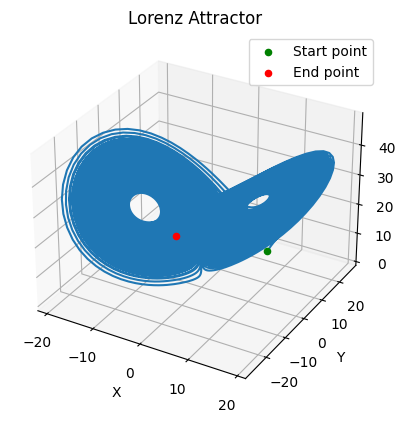
\includegraphics[width=\textwidth]{images/ex4task4_lorenz_1.png}
        \caption{$X_0=[10,10,10]$}
        \label{fig:lorenz_1}
    \end{subfigure}
    \begin{subfigure}[b]{0.45\textwidth}
        \centering
        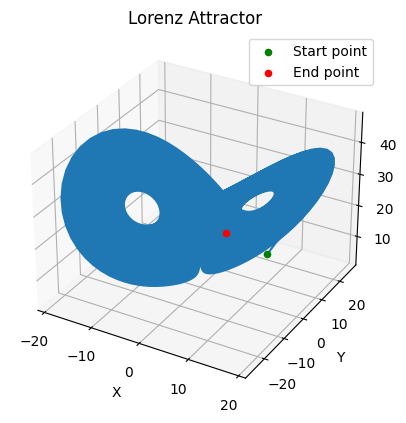
\includegraphics[width=\textwidth]{images/ex4_task4_lorenz_2.png}
        \caption{$\hat{X}_{0}=[10+10^{-8},10,10]$}
        \label{fig:lorenz_2}
    \end{subfigure}
    \caption{Trajectories for different starting points}
    \label{fig:loren_1_2}
\end{figure}

% \begin{figure} [H]
%     \centering
%     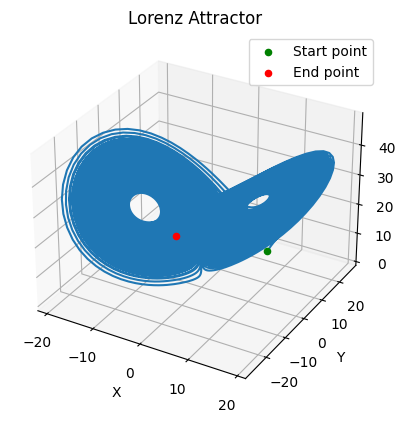
\includegraphics[width=0.5\textwidth]{images/ex4task4_lorenz_1.png}
%     \caption{Trajectory for $X_0=[10,10,10]$}
%     \label{fig:lorenz_1}
% \end{figure}

\item \textbf{Effect of small perturbations:} To study the effects of small perturbations, we plot another trajectory, this time starting the system with a very small perturbation from $\hat{X}_{0}=[10+10^{-8},10,10]$. The rest of the conditions were left the same as previously. The trajectory can be seen in the figure \ref{fig:lorenz_2}. We can clearly see that a very small change in the initial position leads to completely different ending positions, thus solidifying our conclusion from the previous experiment that no two systems starting from different initial conditions will follow each other's trajectories. We also plotted the difference between the two trajectories (${||(x(t)-\hat{x}(t)||}^2$) shown in figure \ref{fig:difference} and recorded the time at which the difference between the two trajectories became larger than 1. From our calculations, we observe that the difference becomes larger than 1 at \textit{24.81} seconds.

\begin{figure} [H]
    \centering
    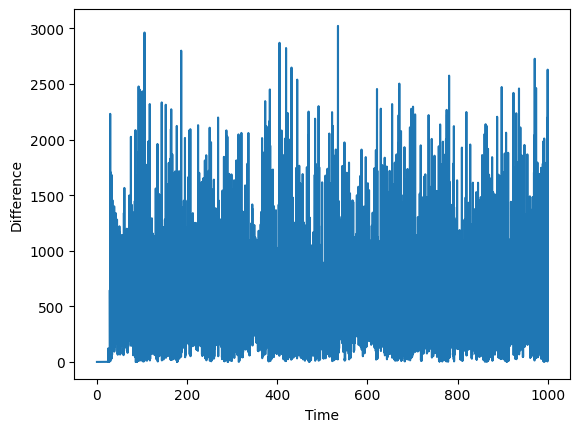
\includegraphics[width=0.5\textwidth]{images/ex4task4_lorenz_3.png}
    \caption{Difference between the two trajectories}
    \label{fig:difference}
\end{figure}

\item \textbf{Effect of $\mathbf{\rho = 0.5}$}: We change one of the parameters $\rho$ to 0.5 and plot the two trajectories again shown in figure \ref{fig:loren_4_5}. We can observe that the trajectories are identical and are probably less sensitive to the initial conditions. The trajectories although are very different from when the $\rho$ value was 28, this indicates that a bifurcation (or multiple ones) occur somewhere between these values.

\begin{figure}[H]
    \centering
    \begin{subfigure}[b]{0.45\textwidth}
        \centering
        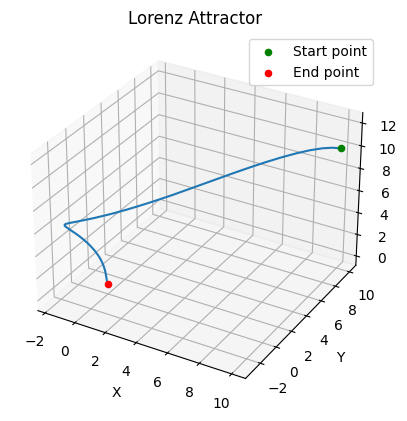
\includegraphics[width=\textwidth]{images/ex4task4_lorenz_4.png}
        \caption{$X_0=[10,10,10]$}
        \label{fig:lorenz_4}
    \end{subfigure}
    \begin{subfigure}[b]{0.45\textwidth}
        \centering
        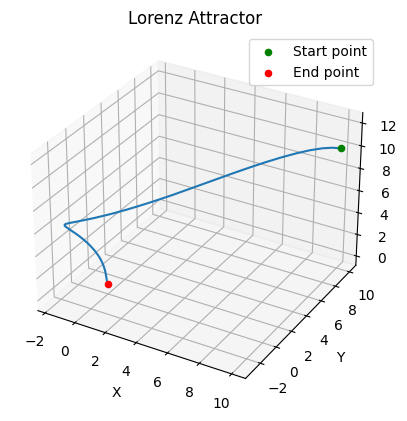
\includegraphics[width=\textwidth]{images/ex4_task4_lorenz_5.png}
        \caption{$\hat{X}_{0}=[10+10^{-8},10,10]$}
        \label{fig:lorenz_5}
    \end{subfigure}
    \caption{Trajectories for different starting points with $\rho$=0.5}
    \label{fig:loren_4_5}
\end{figure}
   \end{itemize}
